\chapter{Implementacija i korisničko sučelje}
		
		
		\section{Korištene tehnologije i alati}
			
			 Komunikacija u timu realizirana je korištenjem aplikacija \underline{WhatsApp}\footnote{https://www.whatsapp.com/} i \underline{Discord}\footnote{https://discord.com/}. Za izradu UML dijagrama korišten je alat \underline{Astah Professional}\footnote{https://astah.net/editions/professional} , a kao sustav za upravljanje izvornim kodom \underline{Git}\footnote{https://git-scm.com/}. Udaljeni repozitorij projekta je dostupan na web platformi \underline{GitLab}\footnote{https://gitlab.com/}.
			 
			 Kao razvojno okruženje korišten je \underline{IntelliJ IDEA}\footnote{https://www.jetbrains.com/idea/} - integrirano razvojno okruženje (IDE) napisano u Javi za razvoj računalnih softvera napisanih u Javi, Kotlinu, Scali, Groovyu i drugim jezicima koji se temelje na JVM-u. Razvio ga je JetBrains (ranije poznat kao IntelliJ) i dostupan je kao Apache 2 licencirano izdanje zajednice (Community Edition) te u vlasničkom komercijalnom izdanju (Ultimate). Oba se mogu koristiti za komercijalni razvoj, a dostupni su za operacijske sustave Windows, macOS i Linux.
			 
			 Aplikacija je napisana koristeći radni okvir \underline{Spring Boot}\footnote{https://start.spring.io/} i jezik \underline{Java}\footnote{https://www.oracle.com/java} za izradu backenda te \underline{React}\footnote{https://reactjs.org/} i jezik \underline{JavaScript}\footnote{https://www.javascript.com/} za izradu frontenda. React, također poznat kao React.js ili ReactJS, je biblioteka u JavaScriptu za izgradnju korisničkih sučelja. Održava je Facebook. React se najčešće koristi kao osnova u razvoju web ili mobilnih aplikacija. Složene aplikacije u Reactu obično zahtijevaju korištenje dodatnih biblioteka za interakciju s API-jem. Spring je radni okvir korišten za olakšan razvoj aplikacija, a omogućava konfiguraciju objekata i lakše upravljanje objektima poslovne logike te općenito brine o kreiranju svih objekata, njihovom povezivanju i čitavom životnom ciklusu. Spring Boot je jedna od komponenti unutar Springa, koja dodatno olakšava njegovo korištenje i omogućava izradu čitavih samostalnih aplikacija. Cilj je ubrzanje i pojednostavljenje razvoja programske potpore.
			 
			 Baza podataka se nalazi na hosting aplikaciji u oblaku, \underline{Render}\footnote{https://render.com/}. Renderova PostgreSQL ponuda olakšava korištenje PostgreSQL-a na siguran, pouzdan i potpuno nesmetan način.\\
			 			
			\eject 
		
	
		\section{Ispitivanje programskog rješenja}
			
			\textbf{\textit{dio 2. revizije}}\\
			
			 \textit{U ovom poglavlju je potrebno opisati provedbu ispitivanja implementiranih funkcionalnosti na razini komponenti i na razini cijelog sustava s prikazom odabranih ispitnih slučajeva. Studenti trebaju ispitati temeljnu funkcionalnost i rubne uvjete.}
	
			
			\subsection{Ispitivanje komponenti}
			\textit{Potrebno je provesti ispitivanje jedinica (engl. unit testing) nad razredima koji implementiraju temeljne funkcionalnosti. Razraditi \textbf{minimalno 6 ispitnih slučajeva} u kojima će se ispitati redovni slučajevi, rubni uvjeti te izazivanje pogreške (engl. exception throwing). Poželjno je stvoriti i ispitni slučaj koji koristi funkcionalnosti koje nisu implementirane. Potrebno je priložiti izvorni kôd svih ispitnih slučajeva te prikaz rezultata izvođenja ispita u razvojnom okruženju (prolaz/pad ispita). }
			
			
			
			\subsection{Ispitivanje sustava}
			
			 \textit{Potrebno je provesti i opisati ispitivanje sustava koristeći radni okvir Selenium\footnote{\url{https://www.seleniumhq.org/}}. Razraditi \textbf{minimalno 4 ispitna slučaja} u kojima će se ispitati redovni slučajevi, rubni uvjeti te poziv funkcionalnosti koja nije implementirana/izaziva pogrešku kako bi se vidjelo na koji način sustav reagira kada nešto nije u potpunosti ostvareno. Ispitni slučaj se treba sastojati od ulaza (npr. korisničko ime i lozinka), očekivanog izlaza ili rezultata, koraka ispitivanja i dobivenog izlaza ili rezultata.\\ }
			 
			 \textit{Izradu ispitnih slučajeva pomoću radnog okvira Selenium moguće je provesti pomoću jednog od sljedeća dva alata:}
			 \begin{itemize}
			 	\item \textit{dodatak za preglednik \textbf{Selenium IDE} - snimanje korisnikovih akcija radi automatskog ponavljanja ispita	}
			 	\item \textit{\textbf{Selenium WebDriver} - podrška za pisanje ispita u jezicima Java, C\#, PHP koristeći posebno programsko sučelje.}
			 \end{itemize}
		 	\textit{Detalji o korištenju alata Selenium bit će prikazani na posebnom predavanju tijekom semestra.}
			
			\eject 
		
		
		\section{Dijagram razmještaja}
			
			Dijagram razmještaja je strukturni statički UML dijagram koji opisuje topologiju sustava i općenito je usredotočen na odnos sklopovskih i programskih dijelova. U ovom slučaju klijent se pomoću web preglednika spaja na korisničko sučelje (frontend) preko kojeg komunicira s poslužiteljskom aplikacijom (backend), a za komunikaciju se koristi protokol HTTPS. Korisničko sučelje  implementirano je koristeći radni okviru React.js i pokrenuto je na platformi Render, dok je poslužiteljska aplikacija također pokrenuta na platformi Render, ali ostvarena je pomoću radnog okvira Spring Boot te pokrenuta unutar kontejnera Docker. Baza podataka, u koju backend aplikacija sprema sve podatke, izvodi se na svome poslužitelju, a nalazi se isto na platformi Render.
			
			\begin{figure}[H]
				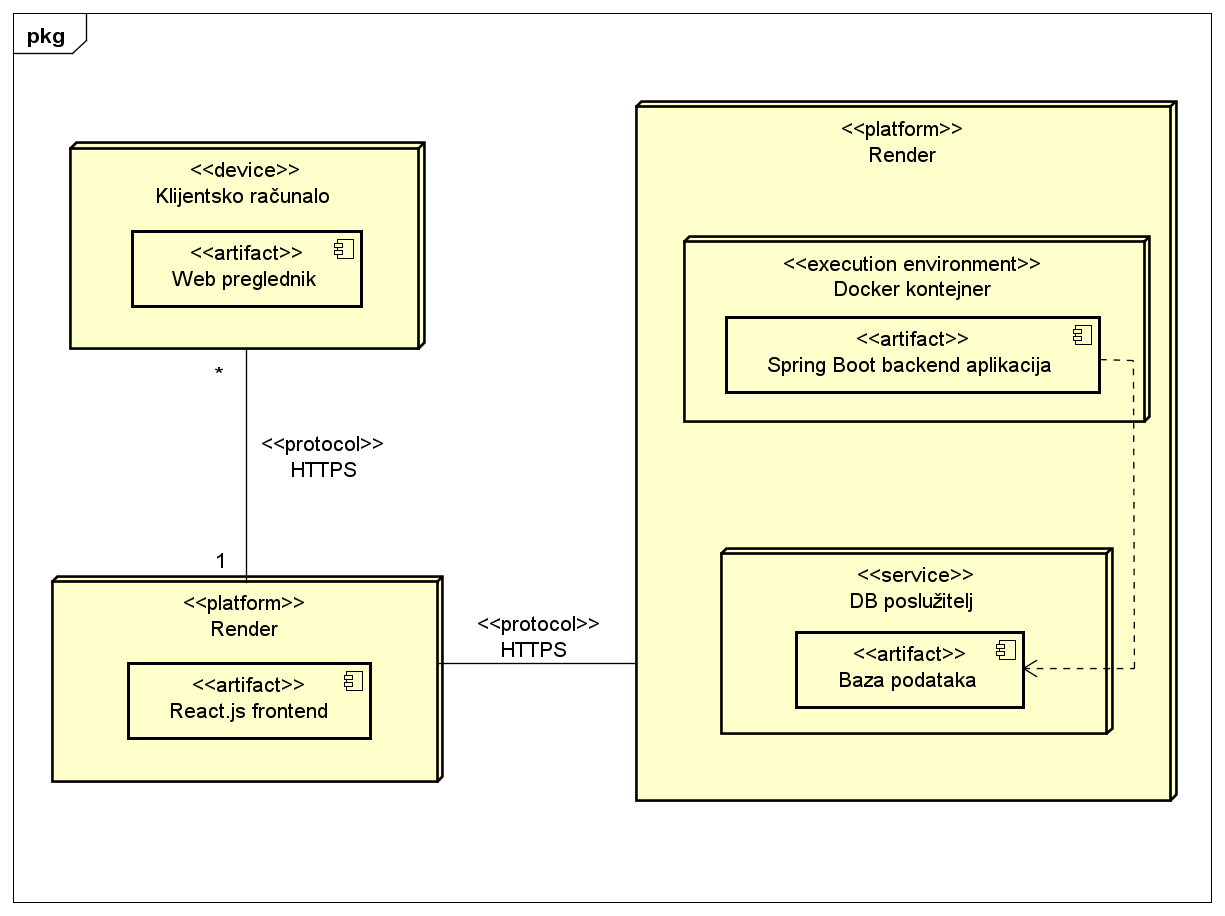
\includegraphics[width=\textwidth]{dijagrami/DeploymentDiagram.PNG} 
				\caption{Dijagram razmještaja}
				\label{fig:DeploymentDiagram}
			\end{figure}
			
			\eject 
		
		\section{Upute za puštanje u pogon}
		
			\textbf{\textit{dio 2. revizije}}\\
		
			 \textit{U ovom poglavlju potrebno je dati upute za puštanje u pogon (engl. deployment) ostvarene aplikacije. Na primjer, za web aplikacije, opisati postupak kojim se od izvornog kôda dolazi do potpuno postavljene baze podataka i poslužitelja koji odgovara na upite korisnika. Za mobilnu aplikaciju, postupak kojim se aplikacija izgradi, te postavi na neku od trgovina. Za stolnu (engl. desktop) aplikaciju, postupak kojim se aplikacija instalira na računalo. Ukoliko mobilne i stolne aplikacije komuniciraju s poslužiteljem i/ili bazom podataka, opisati i postupak njihovog postavljanja. Pri izradi uputa preporučuje se \textbf{naglasiti korake instalacije uporabom natuknica} te koristiti što je više moguće \textbf{slike ekrana} (engl. screenshots) kako bi upute bile jasne i jednostavne za slijediti.}
			
			
			 \textit{Dovršenu aplikaciju potrebno je pokrenuti na javno dostupnom poslužitelju. Studentima se preporuča korištenje neke od sljedećih besplatnih usluga: \href{https://aws.amazon.com/}{Amazon AWS}, \href{https://azure.microsoft.com/en-us/}{Microsoft Azure} ili \href{https://www.heroku.com/}{Heroku}. Mobilne aplikacije trebaju biti objavljene na F-Droid, Google Play ili Amazon App trgovini.}
			
			
			\eject 